% Created 2017-12-04 Mon 09:57
\documentclass[hyperref, UTF-8]{ctexart}
\usepackage{amssymb}
\usepackage{lastpage}
\usepackage{fancyhdr}
\pagestyle{fancy}
\renewcommand{\headrulewidth}{0.4pt} 
\renewcommand{\footrulewidth}{0.4pt}
\usepackage{makeidx}
\usepackage[center]{titlesec} 
\usepackage[colorlinks,
            linkcolor=red,
            anchorcolor=blue,
            citecolor=green
            ]{hyperref}
\usepackage{lastpage}
\fancyhead[LE,RO]{GITC BJ}
\fancyhead[LE,LO]{\thepage}
\fancyfoot[CE,CO]{\leftmark}
\fancyfoot[LE,RO]{\thepage\ of \pageref{LastPage}}
\author{kay}
\title{GITC 2017 BJ \& Comonents}
\makeindex
\begin{document}
\maketitle
\tableofcontents

\section{PPTNote}
\label{sec:orgddc4c40}
\subsection{刘一鸣 Kyligence Apache Kylin 加速大数据 OLAP}
\label{sec:org2b59ba4}
\label{org6fb8a8c}
kylin 的计算以后打算完全基于 spark sql, 不再用 hive
\begin{figure}[htbp]
\centering
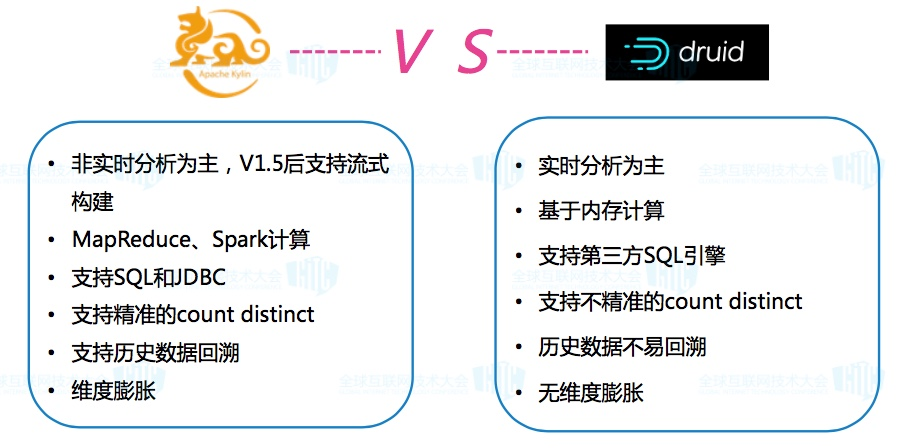
\includegraphics[width=.9\linewidth]{PPTNote/KylinVsDruid_2017-11-29_10-42-52.jpeg}
\caption{kylin 与 druid 对比}
\end{figure}
\subsubsection{优势}
\label{sec:org23a4a23}
\begin{itemize}
\item Apache Kylin: 将 OLAP/DW 带回大数据
\item Apache Kylin 为什么快?
\begin{itemize}
\item 预计算, 空间换时间
\item 将 sort, filter 等操作提升到上边, 将可以预计算的先预计算好, 然后再根据需求过滤排序.
\end{itemize}
\end{itemize}

\subsubsection{遇到的问题}
\label{sec:orgadd7d70}
\begin{itemize}
\item 维度爆炸(多维度组合导致)
\item 结果基于 hbase, 维度的组合作为 rowkey, rowkey 不好设计, 性能有问题, 商业版的不是基于 hbase
\end{itemize}
\subsection{常雷-新一代数据仓库:Apache HAWQ}
\label{sec:org0103c26}
\label{org5ae5bde}
 偶数两大数据仓库/AI 产品  
\begin{itemize}
\item Oushu Database(HAWQ++)
\item Apache HAWQ
\end{itemize}
Oushu Database 4.0: Global Scale: No master, P2P, Geo-replication mixed workload
\subsubsection{数据库的几个阶段}
\label{sec:orgfccc3aa}
\begin{description}
\item[{1960s}] Navigational DBMS (网状 \& 层次模型)
Integrated Data Store (IDS)
Information Management System (IMS)
\item[{1970s}] 1990s: SQL/Relational DBMS
OLTP, Data warehouse, MPP
\item[{2000s}] Present: Post Relational
NoSQL (XML, KV, Graph, Tree), NewSQL, NewDW
\end{description}
\subsubsection{数据库的核心}
\label{sec:org1325250}
\begin{itemize}
\item 数据模型 \& 查询语言
\item 查询优化和执行
\item 索引与存储
\item 事务处理
\end{itemize}
联机分析处理 (OLAP(On-Line Analytical Processing))

联机事务处理 (OLTP(on-line transaction processing))
\subsubsection{数据仓库的演进}
\label{sec:orgbc97b96}
\begin{figure}[htbp]
\centering
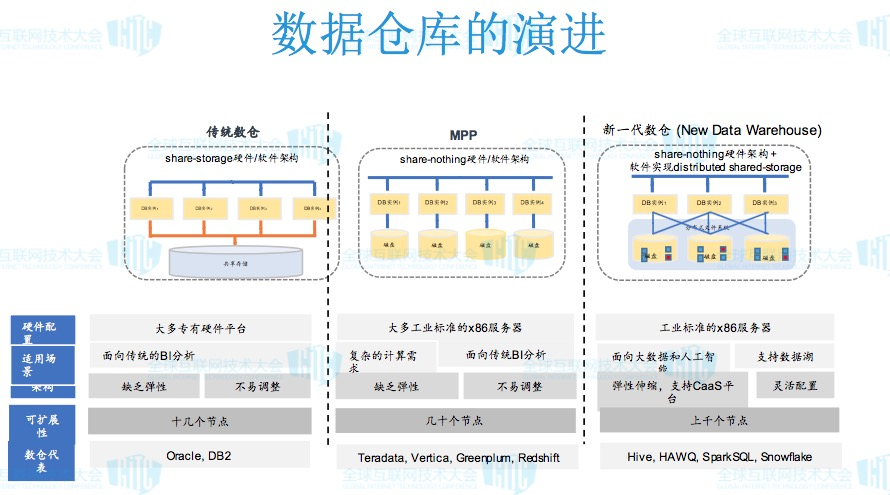
\includegraphics[width=.9\linewidth]{PPTNote/Jietu20171129-133840_2017-11-29_13-38-47.jpg}
\caption{数据仓库的演进}
\end{figure}
\subsubsection{NewDw 细分类别:}
\label{sec:org049e693}
\begin{description}
\item[{Sql on Hadoop}] SparkSql, Hive HAWQ 2.x, Presto
\item[{Sql on Object Store}] Snowflake(on s3), Amazon Athena(on S3)
\item[{Hybrid}] HAWQ 3.x, Oushu, Impala
有自己存储, 对外部存储可插拔
\end{description}

\begin{figure}[htbp]
\centering
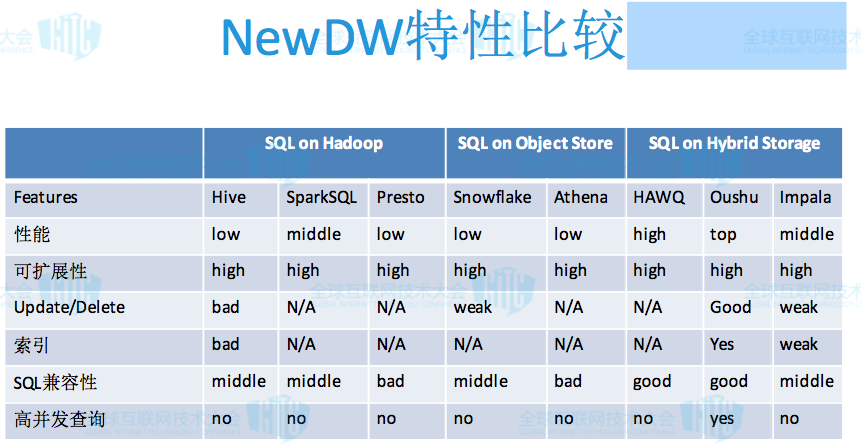
\includegraphics[width=.9\linewidth]{PPTNote/NewDwCompare.jpg}
\caption{New DW 特性比较}
\end{figure}
\subsection{张惠亮 联动大数据处理架构的选择和演进}
\label{sec:org7c33fae}
\begin{enumerate}
\item 用 Zeus 调度任务

在 \url{https://github.com/alibaba/zeus} 没有找到 zeus

\href{https://oschina.net/p/alibaba-zeus}{淘宝 hadoop 作业平台 Zeus oschina}

\href{http://www.cnblogs.com/smartloli/p/4964741.html}{hadoop 任务调度系统比较}

宙斯是一个完整的 Hadoop 的作业平台, 从 Hadoop 任务的调试运行到生产任务的周期调度 宙斯支持任务的整个生命周期
\item 用 datax 传输数据

DataX 是阿里巴巴集团内被广泛使用的离线数据同步工具/平台,实现包括 MySQL、Oracle、HDFS、Hive、OceanBase、HBase、OTS、ODPS 等各种异构数据源之间高效的数据同步功能。
\href{https://github.com/alibaba/DataX}{datax alibaba github}
\end{enumerate}
\subsection{曹永鹏-Mobike 大数据平台建设}
\label{sec:orgfa27ce4}
\subsubsection{平台建设}
\label{sec:org79469b1}
\begin{itemize}
\item 日志收集

Logstash + Kafka + Flume-ng
\item 离线处理

HDFS HA + RM HA / All on Yarn

Hive 数仓

Spark Mllib 模型训练
\item 实时处理
Storm, Spark streaming
\item Es 实时搜索服务
\item 全链路实时监控
\item Yum 源
\item Puppet

配置统一管理

\href{https://puppet.com/products/how-puppet-works}{how-puppet-works}

The result: You get a standard way of automating all of it, at scale.

Puppet, an automated administrative engine for your Linux, Unix, and Windows systems, performs administrative tasks (such as adding users, installing packages, and updating server configurations) based on a centralized specification.
\item Ansible:  自动化部署
\item Zabbix

zabbix 是一个基于 WEB 界面的提供分布式系统监视以及网络监视功能的企业级的开源解决方案。

\href{https://www.zhihu.com/question/19973178}{知乎 开源监控系统中 Zabbix 和 Nagios 哪个更好} 

nagios 最大的亮点是轻量灵活,且报警机制很强,如果你只是需要监控服务器/服务是否在运行,nagios 足矣。

但是如果牵涉到画图方面,我通过这段时间的亲身体会,感觉 nagios+cacti 的结合是不如 zabbix 的 all in one 方式的。
\item Ganglia

Ganglia 和 Nagios,这是两个用于监视数据中心的工具。这两个工具被大量用于高性能计算(HPC)环境中,但是它们对于其他环境也具有很大的吸引力(例如云、呈现集群和托管中心)。此外,两者对监视的定义也采取了不同的侧重点。Ganglia 更多地与收集度量数据并随时跟踪这些数据有关,而 Nagios 一直致力于成为一种报警机制。

\href{https://www.ibm.com/developerworks/cn/linux/l-ganglia-nagios-1/index.html}{用 Ganglia 监视企业集群 (Ganglia 和 Nagios)}

常用开源监视解决方案包括 Cacti、Zenoss、Zabbix、Performance Copilot(PCP)和 Clumon(而且我相信您已经有了自己喜欢的选择)。这些工具(包括 Ganglia 和一些 Nagios 插件)中的许多工具在底层都使用了 RRDTool 或 Tobi Oetiker 的 MRTG(Multi Router Traffic Grapher),以生成漂亮的图形和存储数据。
\end{itemize}
\subsubsection{平台安全}
\label{sec:orgc630cc6}
膜拜: 平台安全: 身份认证: Kerberos, 身份管理: LDAP(轻量级目录访问协议,Lightweight Directory Access Protocol), 访问控制: Sentry, 安全审计, 数据加密
\subsubsection{平台架构}
\label{sec:org8e37c69}
\begin{figure}[htbp]
\centering
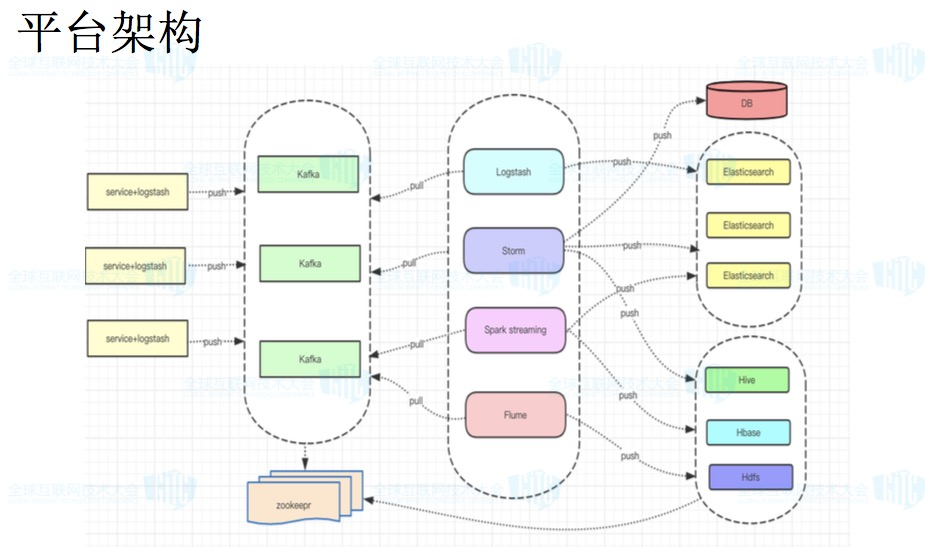
\includegraphics[width=.9\linewidth]{PPTNote/Jietu20171129-151211_2017-11-29_15-14-54.jpg}
\caption{Mobile 平台架构 1}
\end{figure} 
\begin{figure}[htbp]
\centering
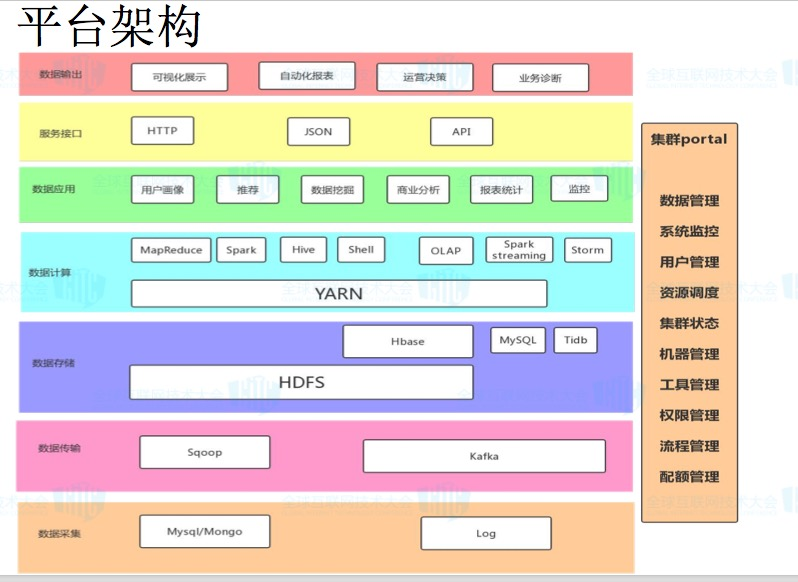
\includegraphics[width=.9\linewidth]{PPTNote/Jietu20171129-151224_2017-11-29_15-15-16.jpg}
\caption{Mobile 平台架构 2}
\end{figure}
\subsection{欧阳辰-实时大数据分析之利器 Druid}
\label{sec:orga1179be}
\label{orgbd98af0}
\begin{itemize}
\item 高可用性,Segment Shard 机制
\item 高性能,亚秒级查询响应
\item 高吞吐,支持实时数据接入,批量数据接入
\item 正确性,lambda 架构能够在 T+1 时间校正实时数据
\item 查询有 segment 级别缓存
\item 堆外内存复用,避免 GC 问题
\end{itemize}

\begin{figure}[htbp]
\centering
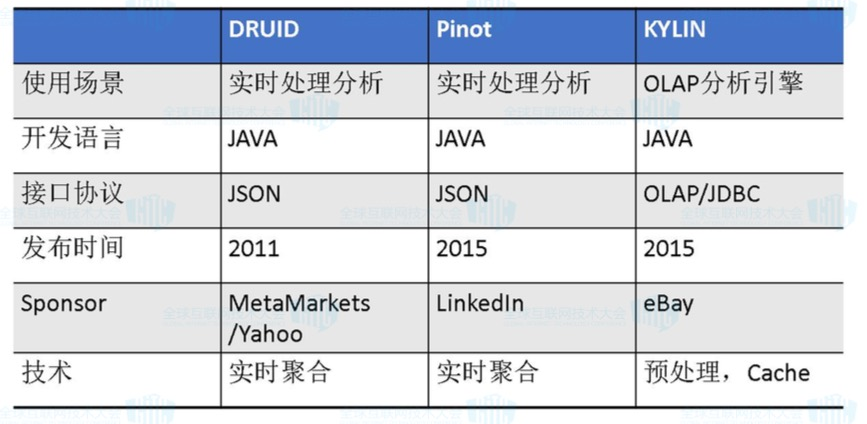
\includegraphics[width=.9\linewidth]{PPTNote/Jietu20171129-160336_2017-11-29_16-04-17.jpg}
\caption{Druid, Pinot, Kylin 对比}
\end{figure}

\subsubsection{Druid 架构图}
\label{sec:org7b0138c}
\begin{figure}[htbp]
\centering
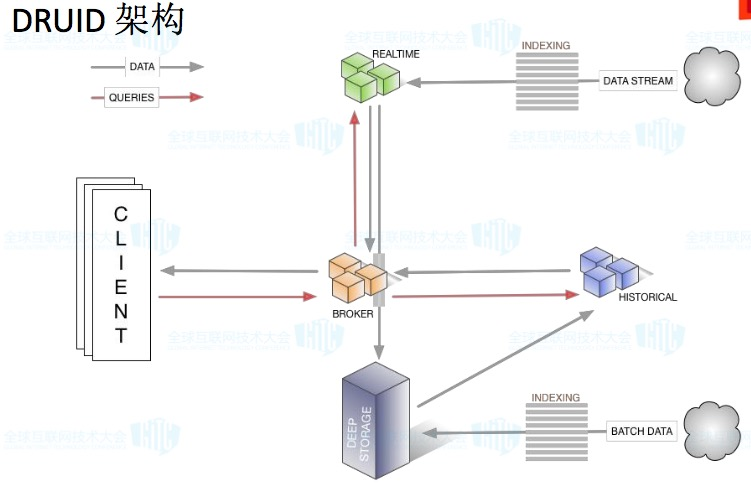
\includegraphics[width=.9\linewidth]{PPTNote/Jietu20171129-154839_2017-11-29_15-49-18.jpg}
\caption{Druid 架构图 1}
\end{figure}

\begin{figure}[htbp]
\centering
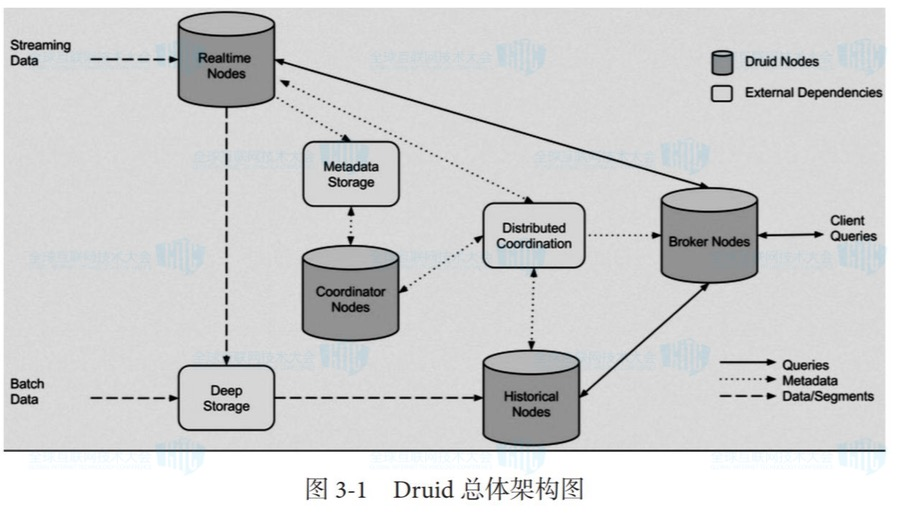
\includegraphics[width=.9\linewidth]{PPTNote/Jietu20171129-154849_2017-11-29_15-50-31.jpg}
\caption{Druid 架构图 2}
\end{figure}

\section{Components}
\label{sec:orge6fe122}
\href{http://www.jdon.com/37625}{CAP 原理和 BASE 思想}
\subsection{Storage}
\label{sec:orgf0504f2}
近几年 OLAP 出现得越来越多,眼花缭乱却又没办法做到一个产品满足所有需求。比如高并发,大吞吐量,SQL Join 等等需求,外加上运维所需要得容错,balance 等,尽管并没有什么黑科技,但在各方面都能达到较好 trade off 的产品其实并不多见。

比如 SQL on Hadoop 系,尽管在存储上已经有很多改进,如早先采用摘要和列存技术的 Parquet,ORCFile,乃至后来引入索引的 CarbonData,以及 SQL 层的工作,如 Impala,Spark SQL 等等,受限于 Hadoop 本身,这些 OLAP 的查询性能有限。 

另一路如 Druid,Pinot,为获得良好的并发性能,这些 OLAP 均引入了预计算以及倒排索引,随之而来的是数据体积的膨胀,对 SQL 的兼容困难,入库能力的降低,以及数据量的限制,此外还有数据入库的原子性等。  

还有些走另类路线的如 Kylin,尽管声称满足了大多数的 OLAP 需求,但在入库实时性,数据膨胀,数据 schema 变更等方面都付出了昂贵的代价,这并不是一个典型面临数据库设计 trade off 的良好工程选择。  

近几年还有一些努力,比如 Clickhouse,Eventql,Indexr,Kudu 等,它们在直面工程 trade off 的路子上做了更多工作,但也各有问题,例如 Clickhouse 无法支撑 auto rebalance,Eventql 缺乏成功经验鲜为人知,Indexr 仍然受限于 hadoop 平台,Kudu 则在 atomic update 上遇到瓶颈,在大规模数据上的性能缺乏保证。  

链接:\url{https://www.zhihu.com/question/63791253/answer/213977376}  

来源:知乎  

著作权归作者所有。商业转载请联系作者获得授权,非商业转载请注明出处。  

\subsubsection{Kudu}
\label{sec:orgc7e9624}
\href{https://oschina.net/news/73633/kudu-apache-hadoop}{Kudu:为大数据快速分析量身定制的 Hadoop 存储系统}   

\href{http://kudu.apache.org/kudu.pdf}{Kudu paper}, 论文中有 Impala-Kudu, Impala-Parquet, Hbase 性能方面的对比   

\href{https://kudu.apache.org/overview.html}{Apache Kudu}   

\href{https://github.com/apache/kudu}{Kudu github}   

\href{http://www.cnblogs.com/lpthread/p/4923183.html}{Cloudera Impala Kudu – 在快数据上的进行快分析的存储}   

A new addition to the open source Apache Hadoop ecosystem, Apache Kudu completes Hadoop's storage layer to enable \textbf{fast analytics on fast data}.   

Kudu:为大数据快速分析量身定制的 Hadoop 存储系统, 对 HDFS 与 Apache HBase 提供的功能进行补充。

Kudu 的目标是:
\begin{itemize}
\item 对于 scan 和随机访问都有非常好的性能,从而降低客户构造混合架构的复杂度
\item 提供快速的全量数据分析与实时处理功能;
\item 充分利用先进 CPU 与 I/O 资源;
\item 既能够支持分析,又能够支持更新、删除和实时查询;
\item 简单、可扩展的数据模型
\end{itemize}

Some of Kudu’s benefits include:
\begin{itemize}
\item Fast processing of OLAP workloads.
\item Integration with MapReduce, Spark and other Hadoop ecosystem components.
\item Tight integration with Apache Impala (incubating), making it a good, mutable alternative to using HDFS with Apache Parquet.
\item Strong but flexible consistency model, allowing you to choose consistency requirements on a per-request basis, including the option for strict-serializable consistency.
\item Strong performance for running sequential and random workloads simultaneously.
\item Easy to administer and manage with Cloudera Manager.
\item High availability. Tablet Servers and Masters use the Raft Consensus Algorithm, which ensures that as long as more than half the total number of replicas is available, the tablet is available for reads and writes. For instance, if 2 out of 3 replicas or 3 out of 5 replicas are available, the tablet is available.  

Reads can be serviced by read-only follower tablets, even in the event of a leader tablet failure.
\item Structured data model.
\end{itemize}

\begin{figure}[htbp]
\centering
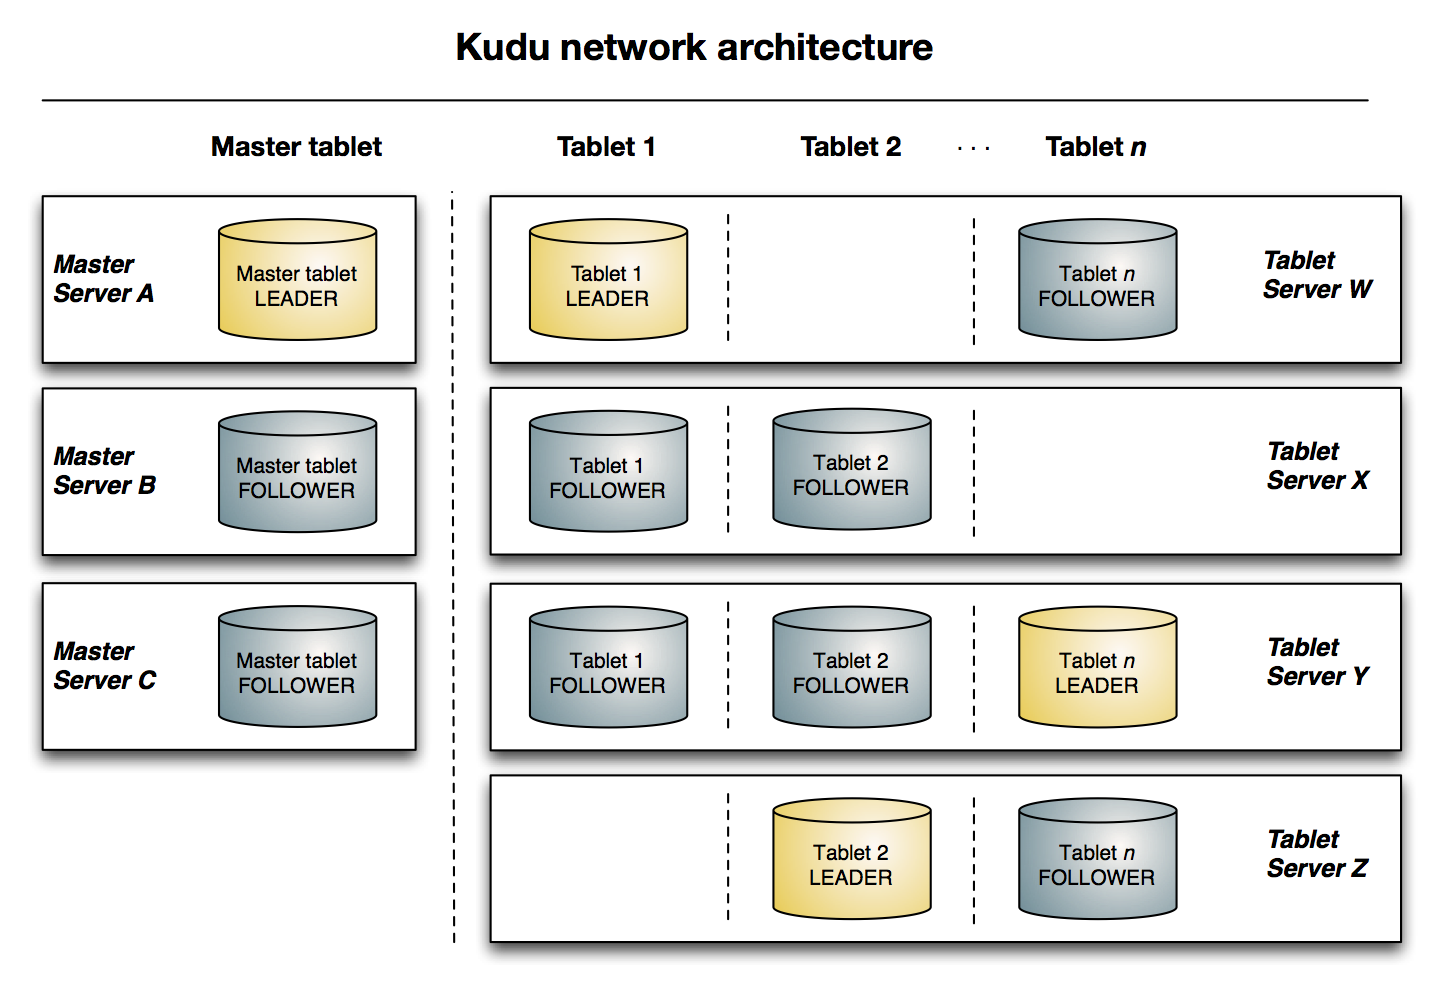
\includegraphics[width=.9\linewidth]{Component/kudu-architecture-2_2017-11-29_17-15-56.png}
\caption{Kudu network architecture}
\end{figure}   

\subsubsection{Hbase}
\label{sec:org7026b65}
\href{http://hbase.apache.org}{Apache Hbase}  

\href{http://blog.csdn.net/woshiwanxin102213/article/details/17584043}{Hbase 原理、基本概念、基本架构} 

\href{https://yq.aliyun.com/articles/60452}{Hbase 系统架构图} 
\paragraph{Hbase 特性}
\label{sec:org579e92d}

\textbf{Features}:
\begin{itemize}
\item Strongly consistent reads/writes
HBase is not an "eventually consistent" DataStore. This makes it very suitable for tasks such as high-speed counter aggregation.
\item Automatic sharding
HBase tables are distributed on the cluster via regions, and regions are automatically split and re-distributed as your data grows.
\item Automatic RegionServer failover
\item Hadoop/HDFS Integration
HBase supports HDFS out of the box as its distributed file system.
\item MapReduce
HBase supports massively parallelized processing via MapReduce for using HBase as both source and sink.
\item Java Client API
HBase supports an easy to use Java API for programmatic access.
\item Thrift/REST API
HBase also supports Thrift and REST for non-Java front-ends.
\item Block Cache and Bloom Filters
HBase supports a Block Cache and Bloom Filters for high volume query optimization.  

Operational Management: HBase provides build-in web-pages for operational insight as well as JMX metrics.
\end{itemize}

Hbase 表的特点:
\begin{itemize}
\item 大:一个表可以有数十亿行,上百万列;
\item 无模式:每行都有一个可排序的主键和任意多的列,列可以根据需要动态的增加,同一张表中不同的行可以有截然不同的列;
\item 面向列:面向列(族)的存储和权限控制,列(族)独立检索;
\item 稀疏:空(null)列并不占用存储空间,表可以设计的非常稀疏;
\item 数据多版本:每个单元中的数据可以有多个版本,默认情况下版本号自动分配,是单元格插入时的时间戳;
\item 数据类型单一:Hbase 中的数据都是字符串,没有类型。
\end{itemize}

Hbase 不适用场景:  事务要求高,多表 Join 查询。 

\paragraph{Hbase 系统架构}
\label{sec:orgf8710f6}


\begin{figure}[htbp]
\centering
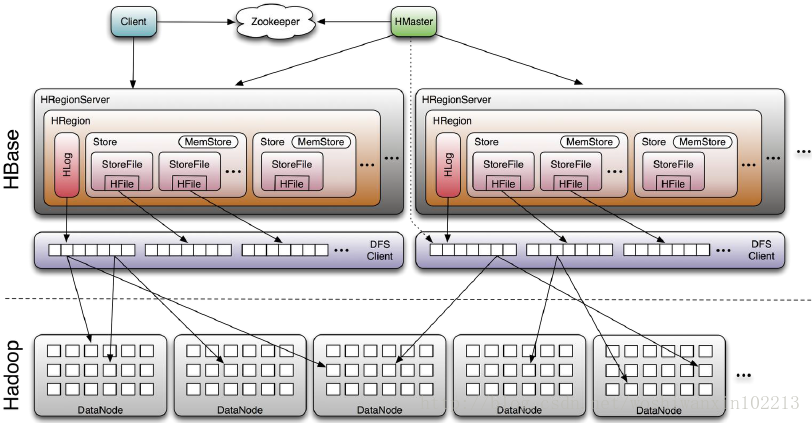
\includegraphics[width=.9\linewidth]{Component/20131226173618000_2017-11-29_19-25-06.png}
\caption{Hbase 系统架构图}
\end{figure}
\subsubsection{Cassandra}
\label{sec:orgb987654}
\href{http://blog.csdn.net/zhangxinrun/article/details/7298601}{Cassandra VS. HBase}   

\href{https://zh.wikipedia.org/zh-hans/Cassandra}{Cassandra 维基百科}    

无中心化, 不存在单点问题.  

二维的 key-value 存储.  

Cassandra 的数据并不存储在分布式文件系统如 GFS 或 HDFS 中,而是直接存于本地。与 BigTable 一样,Cassandra 也是日志型数据库,即把新写入的数据存储在内存的 Memtable 中并通过磁盘中的 CommitLog 来做持久化,内存填满后将数据按照 key 的顺序写进一个只读文件 SSTable 中,每次读取数据时将所有 SSTable 和内存中的数据进行查找和合并。这种系统的特点是 \textbf{写入比读取更快} ,因为写入一条数据是顺序计入 commit log 中,不需要随机读取磁盘以及搜索。 

Cassandra 的系统架构与 Dynamo 类似,是基于一致性哈希的完全 P2P 架构,每行数据通过哈希来决定应该存在哪个或哪些节点中。集群没有 master 的概念,所有节点都是同样的角色,彻底避免了整个系统的单点问题导致的不稳定性,集群间的状态同步通过 Gossip 协议来进行 P2P 的通信。每个节点都把数据存储在本地,每个节点都接受来自客户端的请求。每次客户端随机选择集群中的一个节点来请求数据,对应接受请求的节点将对应的 key 在一致性哈希的环上定位是哪些节点应该存储这个数据,将请求转发到对应的节点上,并将对应若干节点的查询反馈返回给客户端。 

cassandra 是一个大表数据库,优点就是语句很像关系型数据库。 

当你仅仅是存储海量增长的消息数据,存储海量增长的图片,小视频的时候,你要求数据不能丢失,你要求人工维护尽可能少,你要求能迅速通过添加机器扩充存储,那么毫无疑问,Cassandra 现在是占据上风的。  

但是如果你希望构建一个超大规模的搜索引擎,产生超大规模的倒排索引文件(当然是逻辑上的文件,真实文件实际上被切分存储于不同的节点上),那么目前 HDFS+HBase 是你的首选。

Cassandra 使用场景:

\begin{enumerate}
\item 事件记录
由于列族数据库可存放任意数据结构,所以它很适合用来保存应用程序状态或运行中遇到的错误等事件信息。在企业级环境下,所有应用程序都可以把事件写入 Cassandra 数据库。它们可以用 appname:timestamp(应用程序名:时间戳)作为行键,并使用自己需要的列。由于 Cassandra 的写入能力可扩展,所以在事件记录系统中使用它效果会很好。

\item 内容管理系统与博客平台
使用列族,可以把博文的”标签”(tag)、”类别”(category)、”链接”(link)和”trackback”(俗称引用告知,是一种网志工具,它可以让文章作者知道该文读者中有哪些人撰写了哪些与之有关的文章)等属性放在不同的列中。评论信息即可以与上述内容放在同一行,也可以移到另一个”键空间”。同理,博客用户与实际博文亦可存于不同列族中。博客平台:我们储存每个信息到不同的列族中。举个例子,标签可以储存在一个,类别可以在一个,而文章则在另一个
\item 计数器
在网络应用程序中,通常要统计某页面的访问人数并对其分类,以算出分析数据。此时可使用 ConterColumnType 来创建列族。

创建好列族后,可以使用任意列记录网络应用程序中每个用户访问每一页面的次数。

也可以使用 CQL 增加计数器的值。

\item 限期使用
我们可能需要向用户提供试用版,或是在网站上将某个广告条显示一定时间。这些功能可以通过”带过期时限的列”(expiring column)来完成。这种列过了给定时限后,就会又 Cassandra 自动删除。这个时限叫做 TTL(Time To Live,生存时间),以秒为单位。经过 TTL 指定的时长后,这种列就被删掉了。程序若检测到此列不存在,则可收回用户访问权限或移除广告条。
\item 日志。因为我们可以将数据储存在不同的列中,每个应用程序可以将信息写入自己的列族中。
\end{enumerate}

Cassandra 不适合场合:

有些问题是有列族数据库来解决并不是最佳选择,例如需要以”ACID 事务”执行写入及读取操作的系统。如果想让数据库根据查询结果来聚合数据(例如 sum 求和)或 avg(求平均值),那么得把每一行数据都读到客户端,并在此执行操作。

在开发早期原型或开始试探某个技术方案时,不太适合用 Cassandra。开发初期无法确定查询模式的变化情况,而查询模式一旦改变,列族的设计也要随之修改。这将阻碍产品创新团队的工作并降低开发者的生产能力。

在关系型数据库中,数据模式的修改成本很高,而这却降低了查询模式的修改成本;Cassandra 则与之相反,改变其查询模式要比改变数据模式代价更高。

\begin{enumerate}
\item 如果我们需要 ACID 事务。Cassandra 就不支持事务。

\item 原型设计。如果我们分析 Cassandra 的数据结构,我们就会发现结构是基于我们期望的数据查询方式而定。在模型设计之初,我们根本不可能去预测它的查询方式,而一旦查询方式改变,我们就必须重新设计列族。
\end{enumerate}
Cassandra 缺点:
\begin{enumerate}
\item 读的性能太慢无中心的设计,造成读数据时通过逆熵做计算,性能损耗很大,甚至会严重影响服务器运作。
\item 数据同步太慢(最终一致性延迟可能非常大)由于无中心设计,要靠各节点传递信息。相互发通知告知状态,如果副本集有多份,其中又出现节点有宕机的情况,那么做到数据的一致性,延迟可能非常大,效率也很低的。
\item 用插入和更新代替查询,缺乏灵活性,所有查询都要求提前定义好。与大多数数据库为读优化不同,Cassandra 的写性能理论上是高于读性能的,因此非常适合流式的数据存储,尤其是写负载高于读负载的。与 HBase 比起来,它的随机访问性能要高很多,但不是很擅长区间扫描,因此可以作为 HBase 的即时查询缓存,由 HBase 进行批量的大数据处理,由 Cassandra 提供随机查询的接口
\item 不支持直接接入 hadoop,不能实现 MapReduce。现在大数据的代名词就是 hadoop,做为海量数据的框架不支持 hadoop 及 MapReduce,就将被取代。除非 Cassandra 能够给出其他的定位,或者海量数据解决方案。DataStax 公司,正在用 Cassandra 重构 HDFS 的文件系统,不知道是否可以成功。
\end{enumerate}
\subsubsection{ClickHouse}
\label{sec:orgeefefc9}
\href{http://www.jianshu.com/p/4b7d652317bb?from=timeline}{大数据实时分析新神器出世-ClickHouse}   

ClickHouse 是俄罗斯第一大搜索引擎 Yandex 开发的列式储存数据库. 


ClickHouse 作为分析型数据库,有三大特点:
\begin{enumerate}
\item 跑分快
ClickHouse 跑分是 Vertica 的 5 倍快
\item 功能多
ClickHouse 支持数据统计分析各种场景
\item 文艺范
目前 ClickHouse 的限制很多,生来就是为小资服务的  
\begin{itemize}
\item \textbf{目前只支持 Ubuntu 系统}
\item 不提供设计和架构文档,设计很神秘的样子,只有开源的 C++源码
\item 不理睬 Hadoop 生态,走自己的路
\end{itemize}
\end{enumerate}

ClickHouse 与 Druid, Apache Kylin 的区别: ClickHouse 可以支持从原始数据的直接查询,ClickHouse 支持类 SQL 语言,提供了传统关系型数据的便利。 

ClickHouse 的不完美之处:
\begin{itemize}
\item 不支持 Transaction:想快就别想 Transaction
\item 聚合结果必须小于一台机器的内存大小
\item 缺少完整的 Update/Delete 操作
\item 支持有限操作系统, 目前仅仅支持 Ubuntu
\item 不适合典型的 Key-Value 存储
\item 不支持 Blob/Document 类型数据
\item 开源社区刚刚启动,主要是俄语为主
\end{itemize}

ClickHouse 关键功能和应用场景:

\begin{figure}[htbp]
\centering
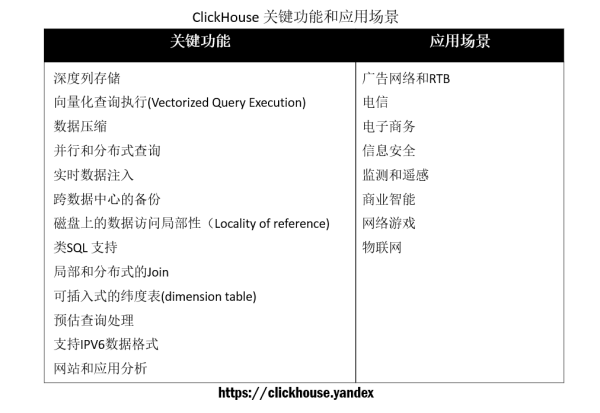
\includegraphics[width=.9\linewidth]{ClickHouse/4410782-be7ecc1aa19372d6_2017-11-30_10-14-41.png}
\caption{关键功能和应用场景(ClickHouse)}
\end{figure}:

\subsubsection{Presto}
\label{sec:org5fae0f3}
\href{http://www.cnblogs.com/tgzhu/p/6033373.html}{Presto 架构及原理}   

\href{http://www.cnblogs.com/hd-zg/p/6904727.html}{实时查询引擎 - Facebook Presto 介绍与应用}   

Presto 的设计和编写完全是为了解决像 Facebook 这样规模的商业数据仓库的交互式分析和处理速度的问题。  

Presto 是 Facebook 推出的一个基于 Java 开发的大数据分布式 SQL 查询引擎, Presto 可以查询包括 Hive、Cassandra 甚至是一些商业的数据存储产品, \textbf{单个 Presto 查询可合并来自多个数据源的数据进行统一分析} 。Presto 的目标是在可期望的响应时间内返回查询结果,Facebook 在内部多个数据存储中使用 Presto 交互式查询,包括 300PB 的数据仓库,超过 1000 个 Facebook 员工每天在使用 Presto 运行超过 3 万个查询,每天扫描超过 1PB 的数据。  

Presto 同样是需要部署到每一个 DataNode 上的分布式系统,它包括一个 coordinator 和多个 worker  

Facebook presto 虽然发展时间不长,版本也还不高,但当前版本在功能上已比较丰富,而且在查询效率上已达到了近乎实时的要求,且非常灵活。Presto 将会成为 \textbf{实时查询工具} 上的一个重要选择。

presto java8 写的,代码质量非常高。设计:纯内存,没有容错,一个 task 失败就整个 query fail。需要注意调整内存相关,线程数等参数,容易 OOM。benchmark 还行。支持标准 SQL.

\begin{figure}[htbp]
\centering
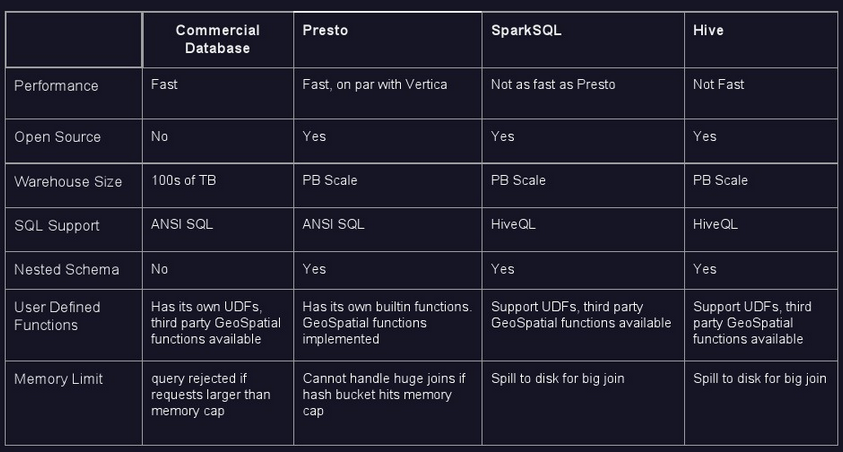
\includegraphics[width=.9\linewidth]{Component/1004194-20161107110246155-560444169_2017-11-30_08-45-32.png}
\caption{presto 与 hive、SparkSQL 对比结果图}
\end{figure}
\subsubsection{Kylin}
\label{sec:org40cd42f}
\hyperref[org6fb8a8c]{内部 PPTNote kylin} 

\href{http://kylin.apache.org/cn/}{APACHE KYLIN™ 概览}  

\href{http://kylin.apache.org/cn/}{APACHE KYLIN™ OVERVIEW EN}
\subsubsection{Druid}
\label{sec:org260574b}
\hyperref[orgbd98af0]{内部 PPTNote Druid}

\href{http://www.cnblogs.com/bonelee/p/6248172.html}{Druid(准)实时分析统计数据库——列存储+高效压缩}   

\href{http://www.csdn.net/article/2014-10-30/2822381/2}{Druid 创始人 Eric Tschetter 详解开源实时大数据分析系统 Druid}  

\href{http://www.open-open.com/lib/view/open1447637905900.html}{Druid 实时数据分析存储系统}   

\href{https://www.2cto.com/database/201610/560087.html}{Druid.io 系列(三):Druid 集群节点}    

\href{https://github.com/druid-io/druid}{druid github}  

\href{http://www.cnblogs.com/lpthread/p/4519687.html}{druid.io 海量实时 OLAP 数据仓库 (翻译+总结) (1)}

\href{http://www.raincent.com/content-85-7091-1.html}{驱动海量大数据实时多维分析,优酷为什么会选择 Druid?}

Druid is a real-time analytics system and is a perfect fit for timeseries and time based events aggregation.  

Druid's storage format is highly optimized for linear scans.  

Druid:是一个实时处理时序数据的 OLAP 数据库,因为它的索引首先按照时间分片,查询的时候也是按照时间线去路由索引。

Druid 是为大型数据集上实时探索查询而设计的开源分析数据存储系统,它的设计意图是在面对代码部署、机器故障以及其他产品系统遇到不测时能保持 100\%正常运行。它也可以用于后台用例,但设计决策明确定位线上服务。

主要特性:
\begin{itemize}
\item 为分析而设计

Druid 是为 OLAP 工作流的探索性分析而构建。它支持各种 filter、aggregator 和查询类型,并为添加新功能提供了一个框架。用户已经利用 Druid 的基础设施开发了高级 K 查询和直方图功能。
\item 交互式查询

Druid 的低延迟数据摄取架构允许事件在它们创建后毫秒内查询,因为 Druid 的查询延时通过只读取和扫描优必要的元素被优化。Aggregate 和 filter 没有坐等结果。
\item 高可用性

Druid 是用来支持需要一直在线的 SaaS 的实现。你的数据在系统更新时依然可用、可查询。规模的扩大和缩小不会造成数据丢失。
\item 可伸缩

现有的 Druid 部署每天处理数十亿事件和 TB 级数据。Druid 被设计成 PB 级别。
\end{itemize}

什么情况下需要 Druid?
\begin{itemize}
\item 当需要在大数据集上面进行快速的,交互式的查询时
\item 当需要进行特殊的数据分析,而不只是简单的键值对存储时
\item 当拥有大量的数据时 (每天新增数百亿的记录、每天新增数十 TB 的数据)
\item 当想要分析实时产生的数据时
\item 当需要一个 24x7x365 无时无刻不可用的数据存储时
\end{itemize}
\subsubsection{Apache HAWQ}
\label{sec:orgb450134}
\hyperref[org5ae5bde]{内部 HAWQ ppt note}

\href{http://www.36dsj.com/archives/36776}{解密 Apache HAWQ ——功能强大的 SQL-on-Hadoop 引擎(有点旧)}  

\href{http://hawq.incubator.apache.org}{Apache HAWQ}  

\href{http://cloud.chinabyte.com/news/99/12558599.shtml}{EMC 讲解 Hawq SQL 性能:左手 Hive 右手 Impala}
\subsubsection{Oushu}
\label{sec:orgce3644d}
新一代数据仓库 :Apache HAWQ 的商业版
\subsubsection{baidu Palo}
\label{sec:orgd6532fe}
\href{https://github.com/baidu/palo}{polo github}   

\href{https://www.zhihu.com/question/63791253}{如何评价百度推出的 Palo,the MPP data warehouse?}  

Palo 的 SQL 基于 Impala  

Palo 特性:
\begin{itemize}
\item 列存
\item SQL 全面兼容
\item 查询优化
\item 必要的 index
\item Atomic Update
\item Schema free
\item Auto Rebalance
\item 多租户
\item 二级切分
\item 基于版本的数据管理(详见 Google Mesa 论文)
\end{itemize}
缺点:
\begin{itemize}
\item 技术亮点不多,大厂开源是得拼指标和技术亮点的(比如 google 的各个系统)
\item 还是和百度云结合太紧密,既然开源了,其他相关生态也得跟上
\item OLAP 中的皇冠:optimizer 功力不足,企业级市场很难接受太多的手动优化 query
\end{itemize}
\subsubsection{Tidb}
\label{sec:orgba86068}
TiDB 是国内 PingCAP 团队开发的一个分布式 SQL 数据库。其灵感来自于 Google 的 F1,TiDB 支持包括传统 RDBMS 和 NoSQL 的特性。  

\href{https://gitee.com/ngaut/tidb}{tidb oschina}  

\href{https://oschina.net/p/tidb}{开源分布式 NewSQL 关系型数据库 TiDB}
\subsubsection{greenplum}
\label{sec:org4cc658b}
\href{http://blog.csdn.net/zx8167107/article/details/78574755}{GreenPlum 博客}   

\href{https://github.com/greenplum-db/gpdb}{gpdb github}   

\href{http://geek.csdn.net/news/detail/49960}{开源大数据引擎:Greenplum 数据库架构分析}   

\href{http://dbaplus.cn/news-21-341-1.html}{聊聊 Greenplum 的那些事}   

分布式关系型 MPP 数据库集群:
\begin{itemize}
\item 支持 PB 级别海量数据存储和处理
\item 主要面向结构化数据、定位服务于 OLAP,大数据计算或分析平台,不擅长做 OLTP
\item 性能好、数据导入高效、开源、随着硬件的增加性能呈线性增长
\item 运维系统完善方便用户使用
\item 查询计划、并行执行
\end{itemize}
Greenplum 主要定位在 \textbf{OLAP} 领域,利用 Greenplum MPP 数据库做大数据计算或分析平台非常适合,例如:数据仓库系统、ODS 系统、ACRM 系统、历史数据管理系统、电信流量分析系统、移动信令分析系统、SANDBOX 自助分析沙箱、数据集市等等。

Greenplum 最大的特点总结就一句话: \textbf{基于低成本的开放平台基础上提供强大的并行数据计算性能和海量数据管理能力} 。这个能力主要指的是并行计算能力,是对大任务、复杂任务的快速高效计算,但如果你指望 MPP 并行数据库能够像 OLTP 数据库一样,在极短的时间处理大量的并发小任务,这个并非 MPP 数据库所长。请牢记,并行和并发是两个完全不同的概念,MPP 数据库是为了解决大问题而设计的并行计算技术,而不是大量的小问题的高并发请求。
\subsubsection{AeroSpike}
\label{sec:org4d81217}
\href{https://en.wikipedia.org/wiki/Aerospike\_database}{Aerospike database}  

\href{https://www.ibm.com/developerworks/cn/analytics/library/ba-aerospike-trs/index.html\%E4\%BB\%A5\%20Aerospike\%20\%E7\%9A\%84\%E5\%86\%85\%E5\%AD\%98\%E9\%80\%9F\%E5\%BA\%A6\%E6\%BB\%A1\%E8\%B6\%B3\%E5\%A4\%A7\%E6\%95\%B0\%E6\%8D\%AE\%E5\%88\%86\%E6\%9E\%90\%E9\%9C\%80\%E6\%B1\%82}{以 Aerospike 的内存速度满足大数据分析需求}   

Aerospike 数据库是一个键-值存储的高性能实时 NoSQL(灵活模式)数据库,以低延迟和高吞吐量而闻名。  

Aerospike 是一个键/值存储,通常被用作缓存,或被用作具有持久性的存储,比如上下文存储。上下文存储可用于:
\begin{itemize}
\item 服务器端会话存储
\item cookie 存储
\item 设备 ID 存储
\item ID 映射
\item 用户首选项或用户配置文件,以便获得实时推荐和个性化 Web 门户上的用户体验
\item 电子商务
\item 旅游网站
\end{itemize}
\subsubsection{Alluxio}
\label{sec:org72b2a6b}
\href{https://www.alluxio.com/blog/alluxiospark-rdd}{使用 Alluxio 高效存储 Spark RDD}   

\href{https://zhuanlan.zhihu.com/p/20624086}{Alluxio : 开源分布式内存文件系统}   

\href{http://www.th7.cn/Program/java/201610/989941.shtml}{spark-alluxio 生产环境的应用与实践}   

Alluxio is a memory speed virtual distributed storage system.Alluxio 是一个开源的基于内存的分布式存储系统,现在成为开源社区中成长最快的大数据开源项目之一。   

由于 Alluxio 的设计以内存为中心,并且是数据访问的中心,所以 Alluxio 在大数据生态圈里占有独特地位,它居于传统大数据存储(如:Amazon S3,HDFS)和大数据计算框架(如 Spark,Hadoop Mapreduce)之间。
\subsubsection{大规模并行处理(MPP)架构}
\label{sec:org072217d}
\begin{enumerate}
\item Master-Slave
\item 无共享架构, 各节点对等
\end{enumerate}
\begin{figure}[htbp]
\centering
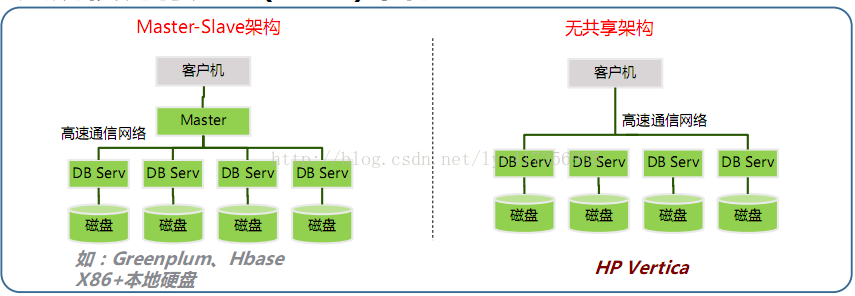
\includegraphics[width=.9\linewidth]{Component/20150413222935866_2017-11-29_10-41-41.png}
\caption{大规模并行处理(MPP)架构}
\end{figure}

\subsubsection{Neo4j}
\label{sec:org5f8296c}
\subsubsection{Redis}
\label{sec:org0e50a15}
\subsubsection{Es}
\label{sec:org3f90fa7}
\subsection{Compute}
\label{sec:org258d79f}
\subsubsection{Flink}
\label{sec:org9e0cef4}
\href{http://www.cnblogs.com/smartloli/p/5580757.html}{Flink 剖析}

\href{https://flink.apache.org}{Apache Flink}

Apache Flink 是一个面向分布式数据 \textbf{流处理和批量数据处理} 的开源计算平台,它能够基于同一个 Flink 运行时(Flink Runtime),提供支持流处理和批处理两种类型应用的功能。  

Flink 包含一下特性:
\begin{itemize}
\item 高吞吐 \& 低延时
\item 支持 Event Time \& 乱序事件
\item 状态计算的 Exactly-Once 语义
\item 高度灵活的流式窗口
\item 带反压的连续流模型
\item 容错性
\item 流处理和批处理共用一个引擎
\item 内存管理
\item 迭代 \& 增量迭代
\item 程序调优
\item 流处理应用
\item 批处理应用
\item 类库生态
\item 广泛集成
\end{itemize}
FLink 与 Spark 它们都支持流式计算,Flink 是一行一行处理,而 Spark 是基于数据片集合(RDD)进行小批量处理,所以 Spark 在流式处理方面,不可避免增加一些延时。Flink 的流式计算跟 Storm 性能差不多,支持毫秒级计算,而 Spark 则只能支持秒级计算。
Flink 是一款新的大数据处理引擎,目标是统一不同来源的数据处理。这个目标看起来和 Spark 和类似。这两套系统都在尝试建立一个统一的平台可以运行批量,流式,交互式,图处理,机器学习等应用。所以,Flink 和 Spark 的目标差异并不大,他们最主要的区别在于实现的细节。
\paragraph{Flink Spark Compare}
\label{sec:orgdc57ac9}

参见 \href{http://www.cnblogs.com/smartloli/p/5580757.html}{Flink 剖析} 2.2 节

Flink 社区没有 Spark 活跃

\subsubsection{spark}
\label{sec:org81ca55d}
\subsubsection{storm}
\label{sec:org8273a74}
\subsubsection{MR}
\label{sec:orgdc19c7f}
\subsection{Monitor}
\label{sec:org9be97eb}
\href{https://addops.cn/post/comparison-to-alternatives.html}{Prometheus 及替代方案对比}

\href{https://prometheus.io/docs/introduction/comparison/}{PROMETHEUS COMPARISON TO ALTERNATIVES}
\subsubsection{OpenTSDB}
\label{sec:orga3ff714}
\href{http://liubin.org/blog/2016/03/05/tsdb-opentsdb/}{时序列数据库武斗大会之 OpenTSDB 篇}

\href{http://www.cnblogs.com/shuiyelifang/p/7909594.html}{OpenTSDB 介绍}

OpenTSDB,可以认为是一个时系列数据(库),它基于 HBase 存储数据,充分发挥了 HBase 的分布式列存储特性,支持数百万每秒的读写,它的特点就是容易扩展,灵活的 tag 机制。
\subsubsection{Prometheus}
\label{sec:org97a50ea}
\href{https://prometheus.io/docs/introduction/overview/}{prometheus docs}

Prometheus's main features are:
\begin{itemize}
\item a multi-dimensional data model with time series data identified by metric name and key/value pairs
\item a flexible query language to leverage this dimensionality
\item no reliance on distributed storage; single server nodes are autonomous
\item time series collection happens via a pull model over HTTP
\item pushing time series is supported via an intermediary gateway
\item targets are discovered via service discovery or static configuration
\item multiple modes of graphing and dashboarding support
\end{itemize}
\subsubsection{Nagios}
\label{sec:org9183aca}
\subsection{Others}
\label{sec:org3462e07}
\subsubsection{Apache Ambari (Hortonworks)}
\label{sec:orgda0ea69}
\href{https://www.ibm.com/developerworks/cn/opensource/os-cn-bigdata-ambari/}{Ambari——大数据平台的搭建利器}   

Apache Ambari 是一种基于 Web 的工具,支持 Apache Hadoop 集群的供应、管理和监控.   

Ambari enables System Administrators to:
\begin{itemize}
\item Provision a Hadoop Cluster
\item Manage a Hadoop Cluster
\item Monitor a Hadoop Cluster
\end{itemize}
Ambari makes Hadoop management simpler by providing a consistent, secure platform for operational control. Ambari provides an intuitive Web UI as well as a robust REST API, which is particularly useful for automating cluster operations. With Ambari, Hadoop operators get the following core benefits:
\begin{itemize}
\item Simplified Installation, Configuration and Management
\item Centralized Security Setup
\item Full Visibility into Cluster Health
\item Highly Extensible and Customizable
\end{itemize}

\subsubsection{Apache Ranger (Hortonworks)}
\label{sec:org38300ef}
\href{http://ranger.apache.org}{Apache Ranger}   

\href{http://www.sohu.com/a/146259668\_465944}{Apache Ranger:Hadoop 生态圈的安全管家}   

\href{http://shenliang1985.blog.163.com/blog/static/2908380520151126102050593/}{Apache Ranger 源码编译及使用介绍}   

Apache ranger 是一个 Hadoop 集群权限框架,提供操作、监控、管理复杂的数据权限,它提供一个集中的管理机制,管理基于 yarn 的 Hadoop 生态圈的所有数据权限。   

Apache Ranger 可以对 Hadoop 生态的组件如 Hive,Hbase 进行细粒度的数据访问控制。通过操作 Ranger 控制台,管理员可以轻松的通过配置策略来控制用户访问 HDFS 文件夹、HDFS 文件、数据库、表、字段权限。这些策略可以为不同的用户和组来设置,同时权限可与 hadoop 无缝对接。   

Apache Ranger 支持以下 HDP 组件的验证、授权、审计、数据加密、安全管理:
\begin{itemize}
\item Apache Hadoop HDFS
\item Apache Hive
\item Apache HBase
\item Apache Storm
\item Apache Knox
\item Apache Solr
\item Apache Kafka
\item YARN
\end{itemize}
\subsubsection{Apache Airflow}
\label{sec:org145e017}
\href{https://oschina.net/p/airflow}{数据管道监控工具 Apache Airflow}
\subsubsection{Zeppelin}
\label{sec:org6160717}
Apache Zeppelin(Apache 开源框架), 是一个让交互式数据分析变得可行的基于网页的 notebook。Zeppelin 提供了数据可视化的框架。
\subsubsection{Kerberos}
\label{sec:org94d0d88}
\subsubsection{Sentry}
\label{sec:org1980f27}
\subsubsection{AI}
\label{sec:orgdf6682a}
Apache Spark 与 TensorFlow 的结合: \href{https://databricks.com/blog/2016/01/25/deep-learning-with-apache-spark-and-tensorflow.html}{Deep Learning with Apache Spark and TensorFlow}
\subsection{Compares}
\label{sec:orgf19f7e8}
OLAP 引擎分类:
\begin{itemize}
\item ROLAP (Relational OLAP)
基于 RDBMS 技术,通过并 化/内存加速计算 • 代表:Presto / Impala / SparkSQL / Drill
\item MOLAP (Multi-dimensional OLAP)
预先聚合明细数据,系统中只存储汇总数据 • 代表:Kylin / Druid
\item Search Engines
基于搜索引擎技术,通过索引加速计算 • 代表:Elasticsearch / Solr
\end{itemize}

\begin{figure}[htbp]
\centering
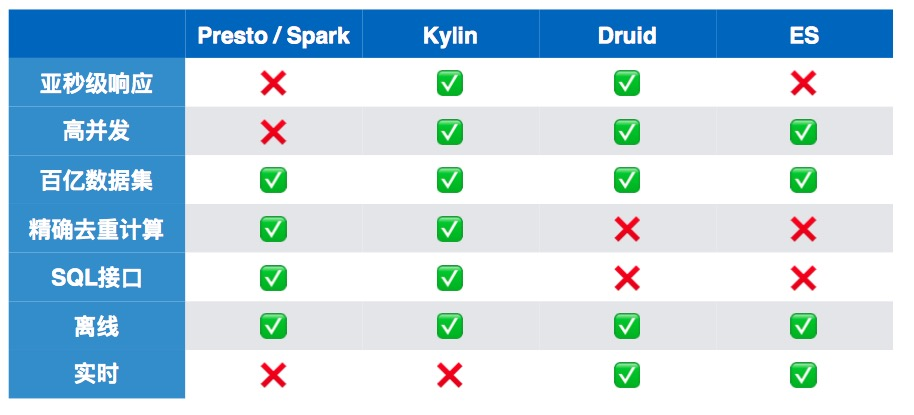
\includegraphics[width=.9\linewidth]{Components/Jietu20171201-174316_2017-12-01_17-43-42.jpg}
\caption{OLAP 引擎对比}
\end{figure}
\subsubsection{Druid vs Impala}
\label{sec:orgdcba50b}
\href{http://druid.io/docs/latest/comparisons/druid-vs-sql-on-hadoop.html}{Druid vs SQL-on-Hadoop (Impala/Drill/Spark SQL/Presto)}

\href{https://github.com/streamlyzer/druidForSL/wiki/Druid-vs-Impala-or-Shark}{Druid vs Impala or Shark}

Impala 不提供存储, Druid 有存储和执行引擎

Druid 和 Impala、Shark 的比较基本上可以归结为需要设计什么样的系统

\begin{enumerate}
\item 设计上:

Druid 被设计用于:
\begin{itemize}
\item 一直在线的服务(be an always on service)
\item 获取实时数据(ingest data in real-time)
\item 处理 slice-n-dice 式的即时查询(handle slice-n-dice style ad-hoc queries)
\end{itemize}
\end{enumerate}
Impala design concerns (as far as I am aware) were to replace Hadoop MapReduce with another, faster, query layer that is completely generic and plays well with the other ecosystem of Hadoop technologies.
\begin{enumerate}
\item 查询速度不同:

Druid 是列存储方式,数据经过压缩加入到索引结构中,压缩增加了 RAM 中的数据存储能力,能够使 RAM 适应更多的数据快速存取。索引结构意味着,当添加过滤器来查询,Druid 少做一些处理,将会查询的更快.  

Impala/Shark 可以认为是 HDFS 之上的后台程序缓存层。 但是他们没有超越缓存功能,真正的提高查询速度。

\item 数据的获取不同:

Druid 可以获取实时数据。  

Impala/Shark 是基于 HDFS 或者其他后备存储,限制了数据获取的速度。

\item 查询的形式不同:

Druid 支持时间序列和 groupby 样式的查询,但不支持 join。  

Impala/Shark 支持 SQL 样式的查询。
\end{enumerate}
\subsubsection{Druid vs Elasticsearch}
\label{sec:org7e6a0a4}

Elasticsearch(ES) 是基于 Apache Lucene 的搜索服务器。它提供了全文搜索的模式,并提供了访问原始事件级数据。Elasticsearch 还提供了分析和汇总支持。根据研究,ES 在数据获取和聚集用的资源比在 Druid 高。

Druid 侧重于 OLAP 工作流程。Druid 是高性能(快速聚集和获取)以较低的成本进行了优化,并支持广泛的分析操作。Druid 提供了结构化的事件数据的一些基本的搜索支持。
\subsubsection{Druid vs Spark}
\label{sec:org7e4d52f}

Spark 是围绕弹性分布式数据集(RDD)的概念,建立了一个集群计算框架,可以被看作是一个后台分析平台。RDD 启用数据复用保持中间结果存在内存中,给 Spark 提供快速计算的迭代算法。这对于某些工作流程,如机器学习,相同的操作可应用一遍又一遍,直到有结果后收敛尤其有益。Spark 提供分析师与不同算法各种各样运行查询和分析大量数据的能力。

Druid 重点是数据获取和提供查询数据的服务,如果建立一个 web 界面,用户可以随意查看数据。

\subsubsection{Druid vs Kudu}
\label{sec:orga6b3e4a}
\href{http://druid.io/docs/latest/comparisons/druid-vs-kudu.html}{Druid vs Kudu}

\href{http://www.ouyangchen.com/wp-content/uploads/2017/03/Meetup-Druid\%E5\%92\%8CKylin\%E5\%9C\%A8\%E7\%BE\%8E\%E5\%9B\%A2\%E7\%82\%B9\%E8\%AF\%84\%E7\%9A\%84\%E9\%80\%89\%E5\%9E\%8B\%E4\%B8\%8E\%E5\%AE\%9E\%E8\%B7\%B5.pdf}{Druid 和 Kylin 在美团点评的选型与实践}

\begin{itemize}
\item Kudu's storage format enables single row updates, whereas updates to existing Druid segments requires recreating the segment, so theoretically the process for updating old values should be higher latency in Druid.
\item Kudu 支持单行更新, Druid 的更新是重建 segments
\item Druid segments 包含 bigmap 索引(可以快速 filtering), kudu 目前不支持
\item Druid segment 架构提供 OLAP 工作流的更快聚合和过滤
\item Druid 添加新数据很快, 但是更新旧的数据有很高的延迟
\item Druid 更擅长于处理连续的不需要频繁更新的事件数据.
\item Kudu 支持任意唯一限制的主键, 并且根据主键查询效率很高
\item Kudu 不包含执行引擎, 意味着在相同的数据上可以支持多个引擎框架(可以用 MR, Spark, SQL); Druid 包含自己的查询层, 运行查询直接下压到数据所在节点聚集计算.
\end{itemize}
\subsubsection{Druid vs Kylin}
\label{sec:orgcd96e96}
\href{http://www.cnblogs.com/dyufei/archive/2009/11/12/2573974.html}{GROUP BY、CUBE 和  ROLLUP 对比}

Druid 是 Rollup,列存储加索引,倒排索引以及 Bitmap 索引。Kudu 主要基于 CUBE, 有维度灾难问题.

Druid 支持实时, Kylin 用于批处理
\subsubsection{Kudu vs Hbase}
\label{sec:org96d0517}
\href{https://bigdata.163.com/product/article/15}{Kudu vs Hbase}

\paragraph{整体架构}
\label{sec:orga8c4088}
\begin{itemize}
\item HBase 的主要组件包括 Master,zookeeper 服务,RegionServer,HDFS
\begin{itemize}
\item Master:用来管理与监控所有的 HRegionServer,也是管理 HBase 元数据的模块。
\item zookeeper:作为分布式协调服务,用于保存 meta 表的位置,master 的位置,存储 RS 当前的工作状态。
\item RegionServer:负责维护 Master 分配的 region,region 对应着表中一段区间内的内容,直接接受客户端传来的读写请求。
\item HDFS:负责最终将写入的数据持久化,并通过多副本复制实现数据的高可靠性。
\end{itemize}
\item Kudu 的主要组件包括 TServer 和 TMaster。
\begin{itemize}
\item TServer:负责管理 Tablet,tablet 是负责一张表中某块内容的读写,接收其他 TServer 中 leader tablet 传来的同步信息。
\item TMaster:集群中的管理节点,用于管理 tablet 的基本信息,表的信息,并监听 TServer 的状态。多个 TMaster 之间通过 Raft 协议实现数据同步和高可用。
\end{itemize}
\item 主要区别
Kudu 结构看上去跟 HBase 差别并不大,主要的区别包括:

(1)Kudu 将 HBase 中 zookeeper 的功能放进了 TMaster 内,Kudu 中 TMaster 的功能比 HBase 中的 Master 任务要多一些。

(2)Hbase 将数据持久化这部分的功能交给了 Hadoop 中的 HDFS,最终组织的数据存储在 HDFS 上。Kudu 自己将存储模块集成在自己的结构中,内部的数据存储模块通过 Raft 协议来保证 leader Tablet 和 replica Tablet 内数据的强一致性,和数据的高可靠性。为什么不像 HBase 一样,利用 HDFS 来实现数据存储,笔者
猜测可能是因为 HDFS 读小文件时的时延太大,所以 Kudu 自己重新完成了底层的数据存储模块,并将其集成在 TServer 中。
\end{itemize}

\paragraph{数据存储方式}
\label{sec:org497f465}

HBase 是一款 Nosql 数据库,典型的 KV 系统,没有固定的 schema 模式,建表时只需指定一个或多个列族名即可,一个列族下面可以增加任意个列限定名。

HBase 将每个列族中的数据分别存储,一个列族中的每行数据中,将 rowkey、列族名、列名、timestamp 组成最终存取的 key 值,另外为了支持修改,删除,增加了一个表征该行数据是否删除的标记。在同一个列族中的所有数据,按照 rowkey:columnfamily:columnQulifier:timestamp 组成的 key 值大小进行升序排列,其中 rowkey、columnfamily、columnQulifier 采用的是字典顺序,其值越大,key 越大,而 timestamp 是值越大,key 越小。HBase 通过按照列族分开存储,相对于行式存储能够实现更高的压缩比,这也是其比较重要的一个特性。

Kudu 是一种完全的列式存储引擎,表中的每一列数据都是存放在一起,列与列之间都是分开的。

为了能够保存一部分历史数据,并实现 MVCC,Kudu 将数据分为三个部分。一个部分叫做 base data,是当前的数据;第二个部分叫做 UNDO records,存储的是从插入数据时到形成 base data 所进行的所有修改操作,修改操作以一定形式进行组织,实现快速查看历史数据;第三个部分是 REDO records,存储的是还未 merge 到当前数据中的更新操作。下图中表示的是在 Kudu 中插入一条数据、更新数据两个操作的做法,当然做法不唯一,不唯一的原因是 Kudu 可以选择先不将更新操作合并到 base data 中。

\paragraph{其它差异}
\label{sec:org7802c91}

HBase:使用的 java,内存的释放通过 GC 来完成,在内存比较紧张时可能引发 full GC 进而导致服务不稳定;

Kudu:核心模块用的 C++来实现,没有 full gc 的风险。
\end{document}